\chapter{Nomenclature}
\label{c:nomenclature}

%------------------------------------------------------------------------
\section{The Known Universe}

The stuff \tao knows about can be divided into 5 categories: 
\begin{example}
  lattice   -- Machine layout and component strengths.
  data      -- For example: orbit, dispersion, coupling etc.
  variables -- For example: steerings, quad strengths, etc.
  plotting  -- How do display stuff.
  global    -- Miscellaneous global parameters.
\end{example}
The \vn{lattice} and \vn{data} stuff are grouped into what is called a
\vn{universe}. The entire collection of \vn{lattice}, \vn{data},
\vn{variables}, \vn{plotting}, and \vn{global} information is called
the \vn{super_universe} and is the sum of what \tao knows about.

%------------------------------------------------------------------------
\subsection{Lattices}


A \vn{lattice} defines the placement of elements in a machine, their
strengths, and the orbit of a beam through them. Each \vn{universe}
has actually three lattices:
  \begin{description}
  \item[Model Lattice]
The strengths or placement of the elements in the \vn{model} lattice
can be varied to see what happens. In particular, things like orbit
correction involve varying things until the \vn{data} as calculated
from the \vn{model} match the \vn{data} as actually measured.
  \item[Design Lattice] 
The \vn{design} lattice is the particular lattice that one wants the
machine to conform to. The strengths of the elements in the \vn{design}
is fixed.
  \item[Base Lattice]
It is sometimes
convenient to designate a reference lattice so that changes in the
\vn{model} from the reference point can be looked at.  This reference lattice
is called the \vn{base}.
  \end{description}

The \vn{model}, \vn{design}, \vn{base} lattices along with any
\vn{data} are bundled together to form what is called a
\vn{universe}. \tao can simultaneously handle multiple universes. Why
is this useful? It can be used, for example, to simulate both rings of
a collider machine. This can be convenient if there are, say, steering
elements in common and it is needed to simultaneously correct the
orbit in both rings. Another example is in a machine where orbits have
been measured under different conditions of, say, beam energy, and it
is desired to fit all the data simultaneously to try to find, say,
rolls in the bends.

%------------------------------------------------------------------------
\subsection{Data}

Blocks of like data are associated with what are called \vn{d1_data}
structures and sets of \vn{d1_data} structures are collected into what
are called \vn{d2_data} structures. For example, a \vn{d1_data}
structure is typically associated with the horizontal data and another
\vn{d1_data} structure is typically associated with the vertical orbit
data. These two structures are then collected into a \vn{d2_data}
structure representing all orbit data. The \vn{d1_data} and
\vn{d2_data} structures are defined in the \tao initialization file
(cf.~Chapter~\ref{c:init}).  When issuing \tao commands one can
specify all the data associated with a \vn{d2_data} structure using
the \vn{d2_data} structure's \vn{name}.  For example the name
\vn{orbit} specifies the orbit data. To specify the data associated
with a \vn{d1_data} structure use the format \vn{d2_name:d1_name}
where \vn{d1_name} is the name of the \vn{d1_data} structure. For
example, if the \vn{d1_data} structure's name for the horizontal orbit
data is \vn{x} then in \tao commands you refer to it by the name
\vn{orbit:x}. Sometimes there is only one \vn{d1_data} structure for a
given \vn{d2_data} structure. In this case the data can be referred to
simply by useing the \vn{d2_data}'s name.

Each data point (for example, the horizontal orbit at some
detector) has a number of quantities associated with it:
  \begin{description}
  \item[Measured Data] 
The data obtained from some measurement. This is generally referred to
as just \vn{data}. When doing lattice design the \vn{data} corresponds to
a constraint (see below).
  \item[Reference Data] 
Reference data obtained from some measurement.
  \item[Model Data]
The data as calculated from the \vn{model} lattice.
  \item[Design Data]
The data as calculated from the \vn{design} lattice.
  \item[Base Data]
The data as calculated from the \vn{base} lattice.
  \end{description}

%------------------------------------------------------------------------
\subsection{Variables}

Blocks of variables are associated with what is called a
\vn{v1_var} structure and each of these structures has a \vn{name}
with which to refer to them in \tao commands. Typically a given variable 
controlls a single attribute of one element in a \vn{model} lattice
of a single universe. However, variables can be configured to simultaneously
control multiple attributes across multiple universes.

Each individual variable has a number of values associated with it:
  \begin{description}
  \item[Measured Value] 
The Value as obtained at the time of the \vn{data} measurement.
  \item[Reference Value] 
The Value as obtained at the time of the \vn{reference} data  measurement.
  \item[Model Value]
The value as given in the \vn{model} lattice.
  \item[Design Value]
The value as given in the \vn{design} lattice.
  \item[Base Value]
The value as given in the \vn{base} lattice.
  \end{description}

%------------------------------------------------------------------------
\section{Plotting}

Some definitions:
\begin{description}
\item[Curve]
A \vn{curve} is a set of (x,y) points to be plotted.
\item[Graph]
A \vn{graph} consists of horizontal and vertical axes along with a set
of \vn{curve}s that are plotted within the graph. 
\item[Plot]
A \vn{plot} is essentially a collection of \vn{graphs}.
\item[Page]
The \vn{page} refers to the x--window where graphics are displayed or the 
corresponding printed graphics page.
\item[Region]
The \vn{page} is divided up into a number of \vn{region}s. 
\end{description}

\begin{figure}
  \centering
  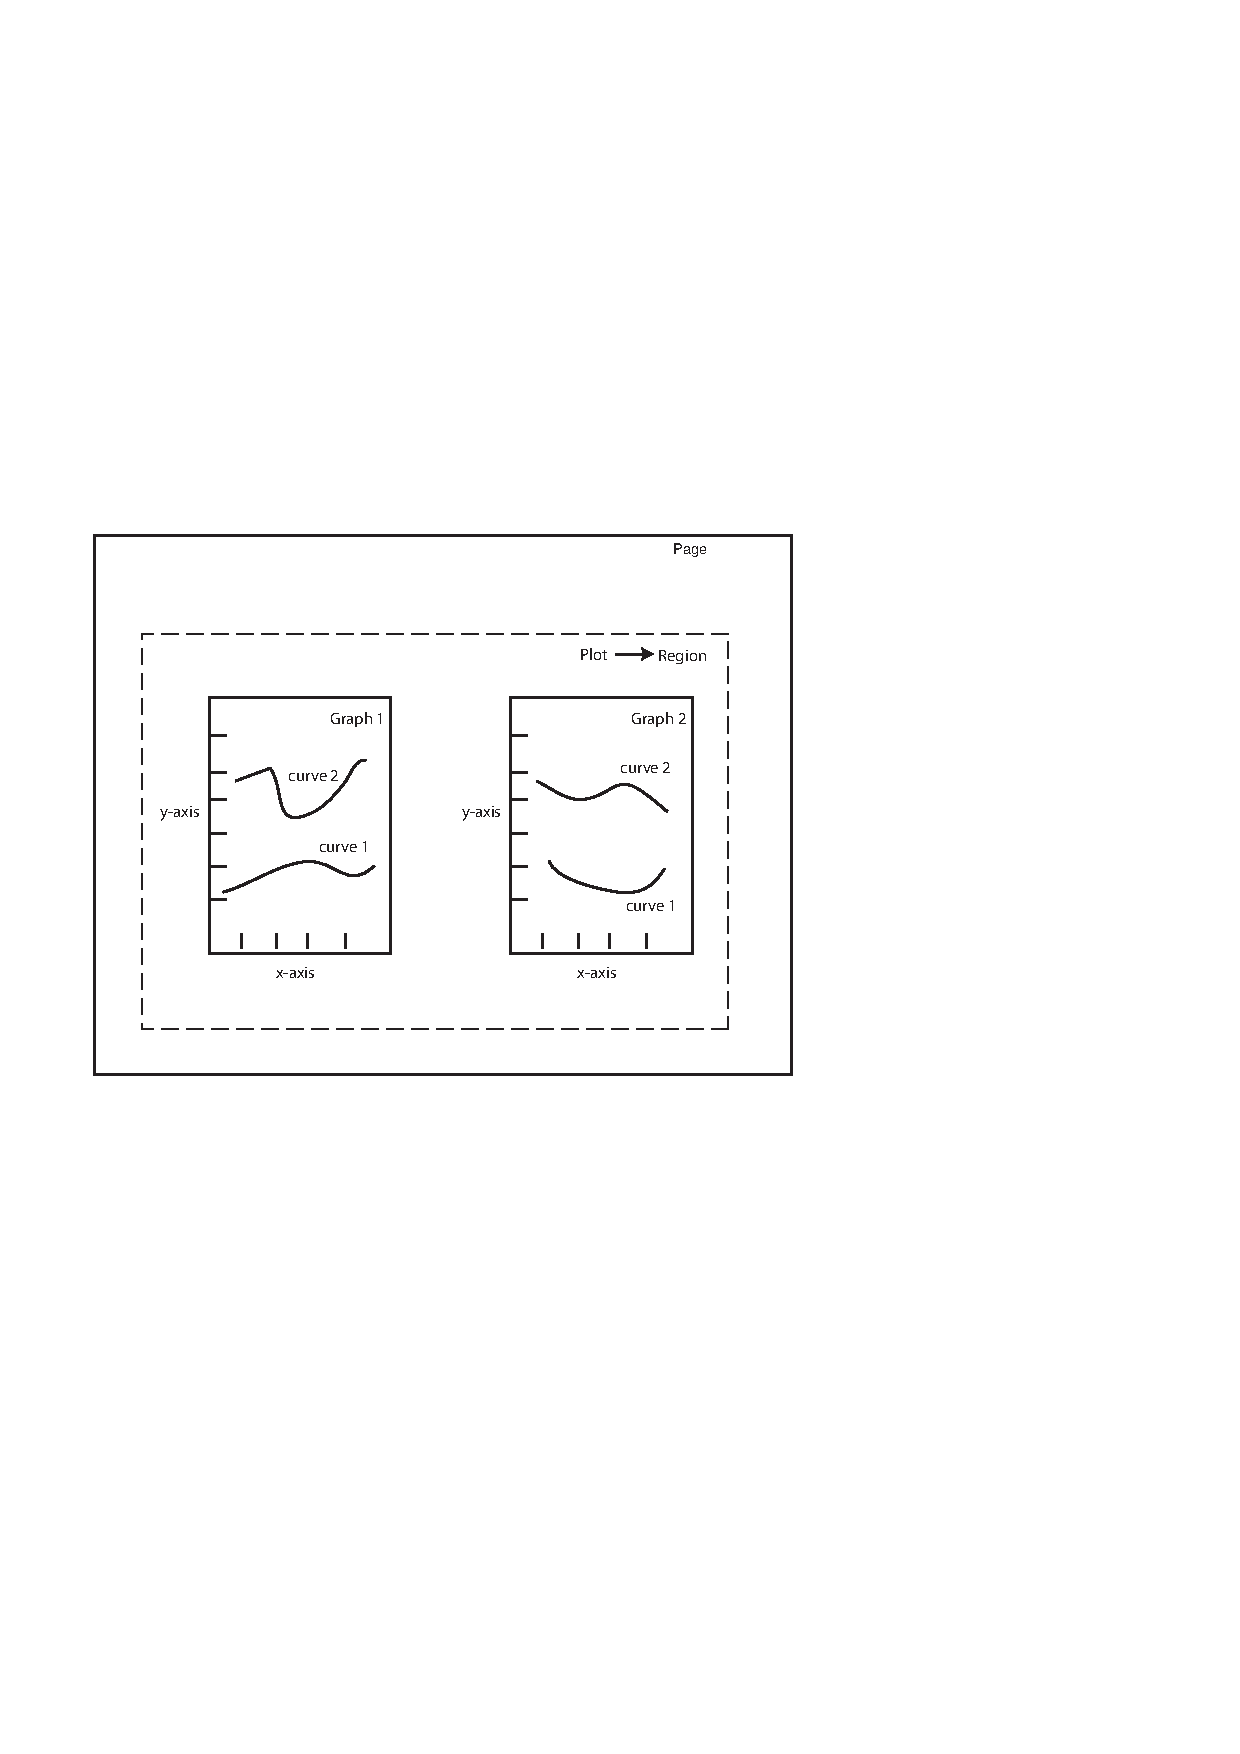
\includegraphics{plot.psfig}
  \caption{A plot has is a collection of graphs and a graph has a 
collection of curves. A plot becomes visible when it 
is associated with a region using the \vn{place} command.}
  \label{f:plot}
\end{figure}

The plot initialization file (cf.~Chapter~\ref{c:init}) defines a set
of \vn{template} plots. A \vn{template} defines what class of data is
plotted (orbit, coupling, etc.), how many \vn{graphs} there are, what
the scales are for the \vn{graph} axes, how the \vn{graph}s are laid
out, etc.  The plot initialization file also defines a set of
\vn{region}s within the \vn{page}.  Using the \vn{place} command one
can assign a particular template to a particular region for plotting.
The relationship between \vn{region}, \vn{plot}, \vn{graph}, and
\vn{curve} is shown graphically in Figure~\ref{f:plot}.

Using the \vn{plot} command one can then specify \vn{who} is
plotted. \vn{who} refers to \vn{measured}, \vn{reference}, \vn{model},
\vn{base}, and/or \vn{design} data.  Notice that the same \vn{template}
plot can be assigned to different \vn{regions} and the plots in different
\vn{regions} can have different scales for their axes or different
\vn{who}.


The \vn{use}, \vn{veto}, \vn{restore},
and \vn{clip} commands are used to display or not to display
individual data points. These are the same commands that control what
data is used in fitting the model to the data. The general rule is
that data that is vetoed for display are simultaneously vetoed for fitting.

When issuing \tao commands, to specify a particular \vn{graph} in a plot
use the notation:
\begin{example}
  region:graph
\end{example}
For example, If a template has two graphs named \vn{x} and \vn{y} and
this template is assigned to the \vn{top} region then the \vn{x} graph
is referred to as \vn{top:x}. 

%------------------------------------------------------------------------
\section{Single Character Input}

Sometimes it is convenient to be able to vary variables using single key strokes
without having to type a carriage return.
With \tao this is possible using what is called \vn{single mode}. This is distinct from
\vn{line mode} where commands to \tao are typed at the command line with a carriage 
return signaling the end of the command. As explained in the initialization chapter
\vn{single mode} uses a special initialization file.

The \vn{single mode} initialization file associates variables with certain keyboard keys
so that when these keys are pressed the value of the variable is varied. This association
between variables and keys is called a \vn{key table}.

